\documentclass[11pt,letterpaper]{article}
\usepackage[margin=0.9in]{geometry}
\usepackage[T1]{fontenc}
\usepackage{lmodern}
\usepackage{microtype}
\usepackage{placeins}
\usepackage{amsmath,booktabs,tabularx}
\usepackage[hidelinks]{hyperref}
\usepackage{xcolor}
\usepackage{tikz}

\usetikzlibrary{arrows.meta,positioning,decorations.pathreplacing,shapes.geometric}
\definecolor{retrievalblue}{HTML}{E8F1FA}
\definecolor{evidenceyellow}{HTML}{FFF3D6}
\definecolor{reportgreen}{HTML}{E7F4EC}
\definecolor{warningred}{HTML}{FCE8E6}
\definecolor{navy}{HTML}{19334A}
\definecolor{sea}{HTML}{245B83}
\definecolor{violet}{HTML}{28604A}
\definecolor{amber}{HTML}{AF650E}
\definecolor{mutedink}{HTML}{4B5563}
\tikzset{panel/.style={draw=black!25,rounded corners=5pt,inner sep=9pt,align=left,font=\small},flow/.style={-{Stealth[length=2mm]},thick,draw=mutedink}}
\usepackage[font=small,labelfont=bf,labelsep=period,justification=raggedright,singlelinecheck=false]{caption}
\setlength{\intextsep}{8pt plus 2pt minus 2pt}
\setlength{\textfloatsep}{10pt plus 2pt minus 2pt}
\captionsetup{skip=6pt}
\setlength{\parskip}{5pt}
\setlength{\parindent}{0pt}
\linespread{1.05}
\setlength{\columnsep}{0.25in}
\setlength{\emergencystretch}{2em}
\newcommand{\draftnote}[1]{\par\smallskip\noindent\textcolor{red!65!black}{\textbf{Draft note.} #1}\par\smallskip}
\hypersetup{pdftitle={Select the Evidence, Then Write: NP at TREC RAGTIME 2026},pdfauthor={Nidhin Pattaniyil, Tanwir Zaman, Semih Yagli},pdflang={en-US}}
\title{Select the Evidence, Then Write\\\large NP at TREC RAGTIME 2026}
\author{Nidhin Pattaniyil \and Tanwir Zaman \and Semih Yagli}
\date{}
\begin{document}
\begin{center}
{\LARGE Select the Evidence, Then Write\par}
\smallskip
{\large NP at TREC RAGTIME 2026\par}
\smallskip
\begin{tabular}{@{}ccc@{}}
Nidhin Pattaniyil & Tanwir Zaman & Semih Yagli\\[2pt]
{\small\href{mailto:npatta01@gmail.com}{\textcolor{sea}{npatta01@gmail.com}}} &
{\small\href{mailto:zaman.tanwir@gmail.com}{\textcolor{sea}{zaman.tanwir@gmail.com}}} &
{\small\href{mailto:semihyagli1@gmail.com}{\textcolor{sea}{semihyagli1@gmail.com}}}
\end{tabular}\\[3pt]
Independent Researchers --- Team NP Labs
\end{center}
\begin{abstract}
We describe a TREC RAGTIME system that writes English reports from multilingual news. It selects factual claims and supporting documents before writing, then checks the output's structure and citation labels. We submitted 102 reports and one abstention. Preliminary organizer assessment on 17 topics gives citation support of 0.9372 and nugget coverage of 0.4343, indicating stronger support for cited statements than coverage of the requested facts.
\end{abstract}

\section{The Task: Answer a Request with a Cited Report}
RAGTIME asks a system to write an English report from news in English, Spanish, Russian, and Chinese~\cite{guidelines}. A request includes a problem statement, background explaining why the report is needed, and a character limit. The output is a sequence of report sentences with citations to original documents. Each cited document must support the entire sentence that cites it.

\begin{figure}[!ht]
\centering
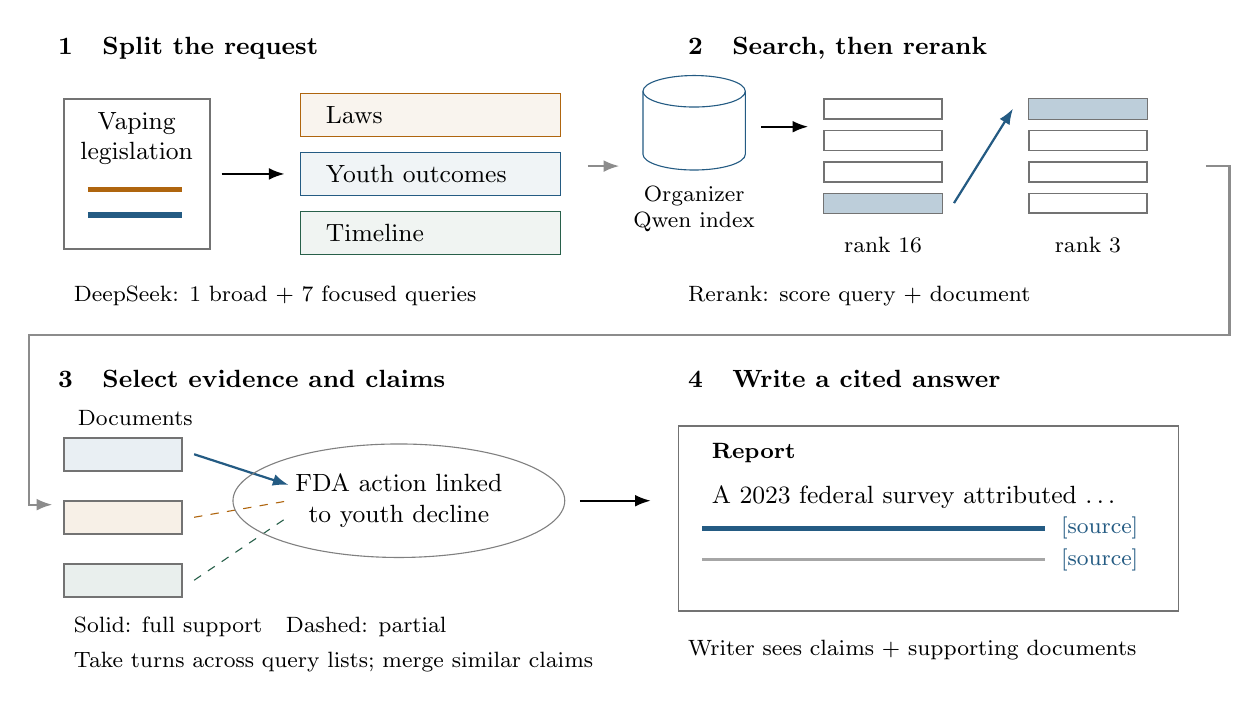
\begin{tikzpicture}[x=1cm,y=1cm,font=\small,
 arr/.style={-{Latex[length=2mm]},line width=.8pt},
 doc/.style={draw=black!55,fill=white,line width=.6pt},
 lab/.style={anchor=west,font=\small\bfseries}]
% One request branches into several query slips.
\node[lab] at (0,0) {1\quad Split the request};
\draw[doc] (.2,-.65) rectangle (2.05,-2.55);
\node[align=center] at (1.12,-1.15) {Vaping\\legislation};
\draw[amber,line width=2pt] (.5,-1.8)--(1.7,-1.8);
\draw[sea,line width=2pt] (.5,-2.12)--(1.7,-2.12);
\draw[arr] (2.2,-1.6)--(3,-1.6);

\foreach \y/\label/\col in {-.85/Laws/amber,-1.6/Youth outcomes/sea,-2.35/Timeline/violet}{
 \draw[\col,fill=\col!7] (3.2,\y-.27) rectangle (6.5,\y+.27);
 \node[anchor=west] at (3.4,\y) {\label};
}
\node[anchor=west,font=\footnotesize] at (.2,-3.15) {DeepSeek: 1 broad + 7 focused queries};
% Separate list outputs, same highlighted article moves up.
\node[lab] at (8,0) {2\quad Search, then rerank};
\draw[sea] (8.2,-.55) ellipse (.65 and .2);
\draw[sea] (7.55,-.55)--(7.55,-1.35) arc (180:360:.65 and .2)--(8.85,-.55);
\node[align=center,font=\footnotesize] at (8.2,-2.05) {Organizer\\Qwen index};
\draw[arr] (9.05,-1)--(9.65,-1);
\foreach \x in {9.85,12.45}{
 \foreach \y in {-.65,-1.05,-1.45,-1.85}{\draw[doc] (\x,\y) rectangle (\x+1.5,\y-.25);}
}
\fill[sea!30] (9.85,-1.85) rectangle (11.35,-2.1);
\fill[sea!30] (12.45,-.65) rectangle (13.95,-.9);
\draw[arr,sea] (11.5,-1.97)--(12.25,-.77);
\node[font=\footnotesize] at (10.6,-2.5) {rank 16};
\node[font=\footnotesize] at (13.2,-2.5) {rank 3};
\node[anchor=west,font=\footnotesize] at (8,-3.15) {Rerank: score query + document};
% Panel ordering and next row.
\draw[arr,black!45] (6.85,-1.5)--(7.25,-1.5);
\draw[arr,black!45] (14.7,-1.5)--(15,-1.5)--(15,-3.65)--(-.25,-3.65)--(-.25,-5.8)--(.05,-5.8);
% Multiple pieces of evidence linked to one retained claim.
\node[lab] at (0,-4.2) {3\quad Select evidence and claims};
\foreach \y/\col in {-4.95/sea,-5.75/amber,-6.55/violet}{
 \draw[doc,fill=\col!10] (.2,\y) rectangle (1.7,\y-.42);
}
\node[anchor=west,font=\footnotesize] at (.25,-4.7) {Documents};
\draw[arr,sea] (1.85,-5.16)--(3.05,-5.55);
\draw[dashed,amber] (1.85,-5.96)--(3.05,-5.75);
\draw[dashed,violet] (1.85,-6.76)--(3.05,-5.95);
\node[draw=black!50,ellipse,align=center,inner sep=5pt] at (4.45,-5.75) {FDA action linked\\to youth decline};
\node[anchor=west,font=\footnotesize] at (.2,-7.35) {Solid: full support\quad Dashed: partial};
\node[anchor=west,font=\footnotesize] at (.2,-7.8) {Take turns across query lists; merge similar claims};
% Writer output is visibly a document with citation marks.
\node[lab] at (8,-4.2) {4\quad Write a cited answer};
\draw[arr] (6.75,-5.75)--(7.65,-5.75);
\draw[doc] (8,-4.8) rectangle (14.35,-7.15);
\node[anchor=west,font=\footnotesize\bfseries] at (8.3,-5.15) {Report};
\node[anchor=west,font=\small] at (8.3,-5.7) {A 2023 federal survey attributed $\ldots$};
\draw[sea,line width=2pt] (8.3,-6.1)--(12.65,-6.1);
\node[text=sea,font=\footnotesize] at (13.35,-6.1) {[source]};
\draw[black!35,line width=1pt] (8.3,-6.5)--(12.65,-6.5);
\node[text=sea,font=\footnotesize] at (13.35,-6.5) {[source]};
\node[anchor=west,font=\footnotesize] at (8,-7.65) {Writer sees claims + supporting documents};
\end{tikzpicture}
\caption{System overview: DeepSeek generates queries, organizer retrieval finds documents, and our system reranks, selects claims, and writes a cited report. Solid and dashed links denote model-assigned full and partial support; document stacks are schematic.}
\label{fig:task}
\end{figure}
\FloatBarrier

We follow Topic 2000, ``Anti-vaping Legislation,'' throughout: a legislative aide needs a report covering the laws and their effects on youth, within 5,000 characters.

\section{From the Request to Search Facets}
We ask \href{https://huggingface.co/deepseek-ai/DeepSeek-V4-Flash}{\textcolor{sea}{DeepSeek v4 Flash}} to break the problem statement and requester background into non-overlapping aspects, called \emph{facets}, and generate focused search queries. It also generates a broad query covering the whole request. The generated queries still overlap in places.

Table~\ref{tab:facets} lists the seven focused queries for Topic 2000. We follow $q_6$, which asks about youth outcomes, through retrieval and writing.

\begin{table}[!ht]
\small\centering
\begin{tabularx}{\linewidth}{@{}lX@{}}
\toprule
Query & Search text\\\midrule
$q_1$ & countries with e-cigarette laws passed dates specific content legal reasoning\\
$q_2$ & electronic cigarette ban sale consumption law date country rationale\\
$q_3$ & vaping regulation effectiveness youth teenagers health outcomes measurable results\\
$q_4$ & e-cigarette parts accessories regulation laws countries dates\\
$q_5$ & legal reasoning behind e-cigarette laws public health youth protection\\
$q_6$ & impact of vaping laws on teenage smoking rates studies\\
$q_7$ & e-cigarette legislation timeline country comparison\\\bottomrule
\end{tabularx}
\caption{Focused queries for Topic 2000, searched alongside the broad query $q_0$.}
\label{tab:facets}
\end{table}

We retain a separate result list for each query.

\section{Find Evidence for Each Part of the Request}
We search each query through the organizer's \href{https://huggingface.co/Qwen/Qwen3-Embedding-8B}{\textcolor{sea}{Qwen-based index}}, then load the returned document IDs from our local corpus copy. We use the supplied English text for synthesis and keep the original document ID for citations.

We use the full document text as evidence for claim extraction and writing.

\textbf{Score and reorder.} The \href{https://huggingface.co/mixedbread-ai/mxbai-rerank-base-v2}{\textcolor{sea}{\texttt{mxbai-rerank-base-v2}}} cross-encoder scores the query together with the document text. Figure~\ref{fig:real-search} follows the survey article from retrieval rank 16 to reranked rank 3. A relevance score ranks evidence; it does not establish factual support.

\textbf{Then, take turns across lists.} We select evidence from each query in rounds, skipping repeated documents. Topic 2000 supplies 24 documents from eight queries, including the survey article in Figure~\ref{fig:real-search}.



\begin{figure}[!ht]
\centering
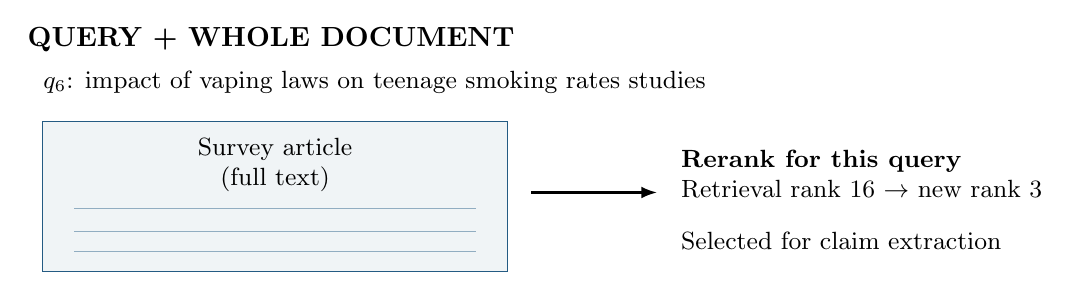
\begin{tikzpicture}[x=1cm,y=1cm,font=\small,txt/.style={anchor=north west,align=left,inner sep=0pt},arr/.style={-{Latex[length=2mm]},line width=.8pt}]
\node[txt,font=\bfseries] at (0,0) {QUERY + WHOLE DOCUMENT};
\node[txt] at (.2,-.55) {$q_6$: impact of vaping laws on teenage smoking rates studies};
\draw[sea,fill=sea!7] (.2,-1.2) rectangle (6.1,-3.1);
\node[align=center] at (3.15,-1.75) {Survey article\\(full text)};
\foreach \y in {-2.3,-2.6,-2.85}{\draw[sea!50] (.6,\y)--(5.7,\y);}
\draw[arr] (6.4,-2.1)--(8,-2.1);
\node[txt] at (8.3,-1.55) {\textbf{Rerank for this query}\\Retrieval rank 16 $\rightarrow$ new rank 3};
\node[txt] at (8.3,-2.6) {Selected for claim extraction};


\end{tikzpicture}
\caption{The cross-encoder scores the query and full survey article together. Reranking moves the article from rank 16 to rank 3; it is then selected for claim extraction.}
\label{fig:real-search}
\end{figure}
\FloatBarrier

\section{Select Claims and Generate the Report}
\subsection{Select claims with supporting documents}
A \emph{nugget} is a factual claim extracted from a document. We use \href{https://github.com/castorini/nuggetizer}{\textcolor{sea}{Nuggetizer}}~\textcolor{sea}{\cite{greatnuggetrecall}} to extract claims, assign full, partial, or no support to claim--document pairs, and retain source links. The model labels support as full if the document supports the entire claim, or partial if it supports only part.

We merge similar claims to reduce repetition, preserving their wording variants and source links. A document becomes eligible for the writer when Nuggetizer labels it as fully supporting at least one retained claim (Figure~\ref{fig:support-routing}).

\begin{figure}[!ht]
\centering
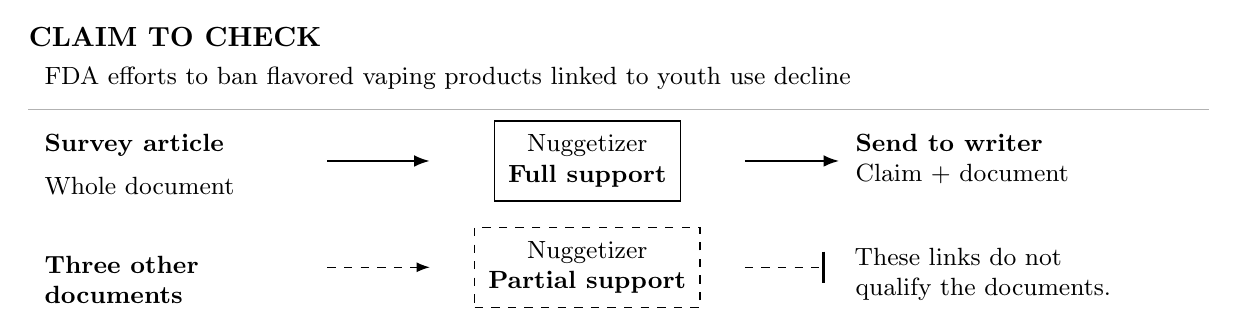
\begin{tikzpicture}[x=1cm,y=1cm,font=\small,txt/.style={anchor=north west,align=left,inner sep=0pt},arr/.style={-{Latex[length=2mm]},line width=.8pt}]
\node[txt,font=\bfseries] at (0,0) {CLAIM TO CHECK};
\node[txt,text width=14.9cm] at (.2,-.5) {FDA efforts to ban flavored vaping products linked to youth use decline};
\draw[black!30] (0,-1.05)--(15,-1.05);
\node[txt] at (.2,-1.35) {\textbf{Survey article}};
\node[txt] at (.2,-1.9) {Whole document};
\draw[arr] (3.8,-1.7)--(5.1,-1.7);
\node[draw,inner sep=5pt,align=center] at (7.1,-1.7) {Nuggetizer\\\textbf{Full support}};
\draw[arr] (9.1,-1.7)--(10.3,-1.7);
\node[txt] at (10.5,-1.35) {\textbf{Send to writer}\\Claim + document};
\node[txt] at (.2,-2.9) {\textbf{Three other}\\\textbf{documents}};
\draw[dashed,-{Latex}] (3.8,-3.05)--(5.1,-3.05);
\node[draw,dashed,inner sep=5pt,align=center] at (7.1,-3.05) {Nuggetizer\\\textbf{Partial support}};
\draw[dashed] (9.1,-3.05)--(10.1,-3.05);
\draw[thick] (10.1,-2.85)--(10.1,-3.25);
\node[txt,text width=4.4cm] at (10.5,-2.8) {These links do not\\qualify the documents.};
\end{tikzpicture}
\caption{Support determines which sources the writer receives. For this claim, Nuggetizer labels the survey article as full support and three other documents as partial support. A partial-support document can still qualify through a full-support link to another retained claim.}
\label{fig:support-routing}
\end{figure}

Claims without a fully supporting source are omitted. If no claim has a citable source, the system abstains.

\subsection{From the writer's input to the final answer}
The writer receives the request, retained claims, and supporting documents, then returns sentences with citation labels (Figure~\ref{fig:writer}). We map those labels to original document IDs for submission.

\begin{figure}[!ht]
\centering
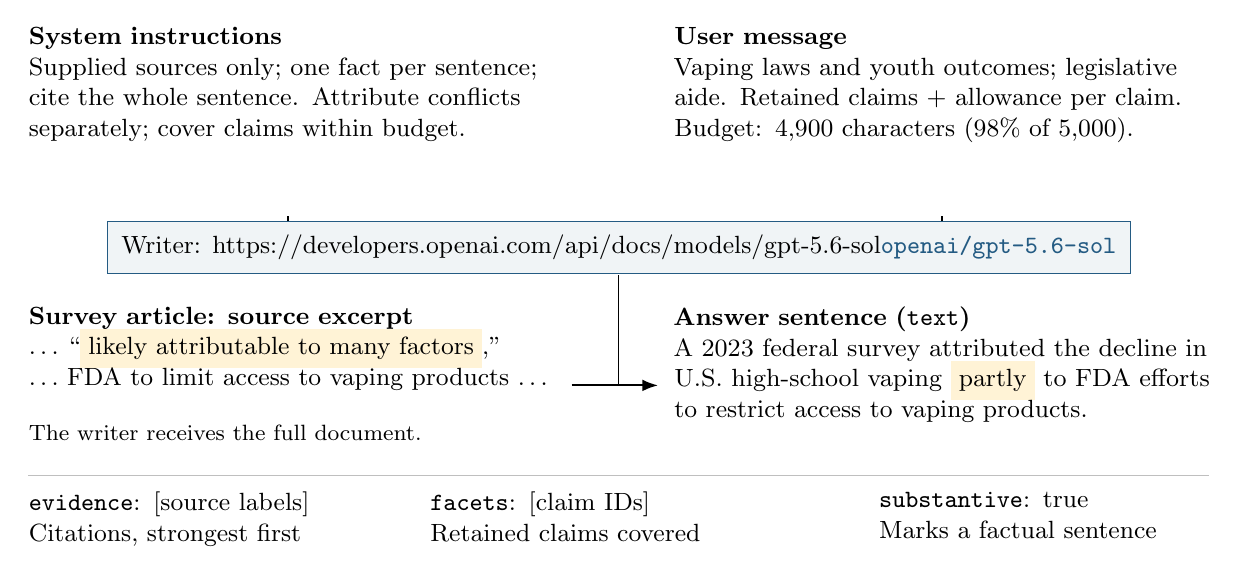
\begin{tikzpicture}[x=1cm,y=1cm,font=\small,
 txt/.style={anchor=north west,align=left,inner sep=0pt},arr/.style={-{Latex[length=2mm]},line width=.8pt}]
\node[txt,text width=6.8cm] at (0,0) {\textbf{System instructions}\\Supplied sources only; one fact per sentence; cite the whole sentence. Attribute conflicts separately; cover claims within budget.};
\node[txt,text width=6.8cm] at (8.2,0) {\textbf{User message}\\Vaping laws and youth outcomes; legislative aide. Retained claims + allowance per claim.\\Budget: 4,900 characters (98\% of 5,000).};
\draw[arr] (3.3,-2.40)--(3.3,-2.80)--(4.4,-2.80);
\draw[arr] (11.6,-2.40)--(11.6,-2.80)--(10.6,-2.80);
\node[draw=sea,fill=sea!7,inner sep=5pt] at (7.5,-2.80) {Writer: \href{https://developers.openai.com/api/docs/models/gpt-5.6-sol}{\textcolor{sea}{\texttt{openai/gpt-5.6-sol}}}};
\draw (7.5,-3.15)--(7.5,-4.55);
\node[txt,text width=6.8cm] at (0,-3.55) {\textbf{Survey article: source excerpt}\\$\ldots$ ``\colorbox{evidenceyellow}{likely attributable to many factors},''\\$\ldots$ FDA to limit access to vaping products $\ldots$};
\node[txt,font=\footnotesize] at (0,-5.05) {The writer receives the full document.};
\draw[arr] (6.9,-4.55)--(8,-4.55);
\node[txt,text width=6.8cm] at (8.2,-3.55) {\textbf{Answer sentence (\texttt{text})}\\A 2023 federal survey attributed the decline in U.S. high-school vaping \colorbox{evidenceyellow}{partly} to FDA efforts to restrict access to vaping products.};
\draw[black!25] (0,-5.70)--(15,-5.70);
\node[txt,text width=4.8cm] at (0,-5.90) {\texttt{evidence}: [source labels]\\Citations, strongest first};
\node[txt,text width=5.3cm] at (5.1,-5.90) {\texttt{facets}: [claim IDs]\\Retained claims covered};
\node[txt,text width=4.3cm] at (10.8,-5.90) {\texttt{substantive}: true\\Marks a factual sentence};
\end{tikzpicture}
\caption{From the survey article to one entry in \texttt{sentences[]}. The answer's ``partly'' preserves the source's qualification; the \texttt{evidence} field links the sentence to its source. Bracketed labels illustrate the output fields.}
\label{fig:writer}
\end{figure}

We reject invalid citation labels, repeated sentences, and factual sentences without citations.

\FloatBarrier

\section{Submitted Output and Evaluation}
We submitted \texttt{np-nugget-sol-v1} on August 13, 2026: 102 reports and one abstention across 103 requests. Reports fit within the 5,000-character limit: the median length was 3,573 characters and the longest was 4,877, excluding citation metadata.

\paragraph{Preliminary organizer results.}
Our citation and sentence support match the reported maxima; nugget coverage and F1 are above the medians but below the maxima (Table~\ref{tab:organizer-results}). The 17-topic assessment is mostly human, with AutoARGUE filling missing citation judgments; the 34-topic assessment uses AutoARGUE throughout.

\begin{table}[!ht]
\centering\renewcommand{\arraystretch}{1.12}
\begin{tabular}{@{}lrrrrrr@{}}
\toprule
& \multicolumn{3}{c}{Mostly human (17 topics)} & \multicolumn{3}{c}{AutoARGUE (34 topics)}\\
\cmidrule(lr){2-4}\cmidrule(l){5-7}
Metric & \textbf{Our run} & Median & Max & \textbf{Our run} & Median & Max\\
\midrule
Citation support & \textbf{0.9372} & 0.8155 & 0.9372 & \textbf{0.9573} & 0.7532 & 0.9573\\
Sentence support & \textbf{0.9344} & 0.7971 & 0.9344 & \textbf{0.9581} & 0.7550 & 0.9581\\
Nugget coverage & \textbf{0.4343} & 0.3581 & 0.4763 & \textbf{0.3916} & 0.3534 & 0.4940\\
F1 & \textbf{0.5715} & 0.4653 & 0.6093 & \textbf{0.5559} & 0.4436 & 0.6121\\
\bottomrule
\end{tabular}
\caption{Preliminary organizer scores (November 4) for \texttt{np-nugget-sol-v1}, on a 0--1 scale; higher is better. Median and max cover 29 runs. Organizer aggregates use \texttt{\_llmfilled} metrics for mostly-human assessment and \texttt{\_micro} for AutoARGUE.}
\label{tab:organizer-results}
\end{table}

Citation support measures whether cited documents support their sentences; sentence support requires every citation to support the sentence. Nugget coverage measures reference facts recovered in supported sentences. The evaluations cover different topic sets, so their scores should be read separately.

\begin{samepage}
\paragraph{When the system abstained.}
Topic 2023, ``The Joyce Hatto Scam,'' asks how beliefs about an artist influence our perception of art, focusing on recordings falsely attributed to the pianist Joyce Hatto. The requester is a classical-music enthusiast who had admired and collected her CDs. None of the selected documents qualified as a supporting source, so the system returned:
\begin{quote}
``Insufficient citation-ready evidence was available to produce a supported report.''
\end{quote}
This was the only abstention among 103 requests. It shows the source-selection rule in action: when no document qualifies, the system declines to answer. It does not establish that the collection lacks relevant information.

\end{samepage}

\section{Limitations}
The method can lose useful facts during retrieval, translation, extraction, or merging. Full-support labels can be wrong, and the final writer can attach a valid label to unsupported wording.

\begin{samepage}
\section{Conclusion}
Our system searches several aspects of a request, selects claims with supporting documents, and writes a cited report from that evidence. It produced 102 reports and declined one request without a qualifying source. Preliminary organizer results show high citation support, with room to improve fact coverage.

\end{samepage}

\paragraph{Use of AI tools.}
Codex assisted with drafting, revision, and figure preparation.

\begin{thebibliography}{9}
\bibitem{guidelines}
TREC RAGTIME organizers.
\emph{TREC 2026 RAGTIME Track Guidelines}.
Version 1, March 23, 2026. Accessed October 3, 2026.
\href{https://docs.google.com/document/d/1XqypNTHxIdazxfnUebrp-EsUuGNhodhQGrJIDnYGaB4/edit}{Official guidelines}.

\bibitem{greatnuggetrecall}
Ronak Pradeep, Nandan Thakur, Shivani Upadhyay, Daniel Campos, Nick Craswell, and Jimmy Lin.
\href{https://doi.org/10.1145/3726302.3730090}{\textcolor{sea}{The Great Nugget Recall: Automating Fact Extraction and RAG Evaluation with Large Language Models}}.
In \emph{Proceedings of SIGIR}, pages 180--190, 2025.

\end{thebibliography}
\appendix
\section{Models and Settings}
\label{sec:settings}
Table~\ref{tab:models} lists the models and settings used at each stage.

\begin{table}[!ht]
\small
\begin{tabularx}{\linewidth}{@{}lX@{}}
\toprule
Stage & Component and role\\\midrule
Query planning & \texttt{deepseek/deepseek-v4-flash-20260423} (\href{https://huggingface.co/deepseek-ai/DeepSeek-V4-Flash}{\textcolor{sea}{model card}}); one broad query and focused facet queries.\\
Hosted retrieval & Organizer-provided \texttt{ragtime2}; Qwen3-Embedding-8B (\href{https://huggingface.co/Qwen/Qwen3-Embedding-8B}{\textcolor{sea}{model card}}), FAISS, and RoutIR. We did not build this retrieval index.\\
Reranking & \texttt{mixedbread-ai/mxbai-rerank-base-v2} (\href{https://huggingface.co/mixedbread-ai/mxbai-rerank-base-v2}{\textcolor{sea}{model card}}); scores query--evidence relevance.\\
Claim selection & Nuggetizer 0.0.5 (\href{https://github.com/castorini/nuggetizer}{\textcolor{sea}{library}}; \href{https://doi.org/10.1145/3726302.3730090}{\textcolor{sea}{paper}}); full-support links make documents citable. Similar claims merge at cosine 0.92 with numeric and negation checks.\\
Writing & \texttt{openai/gpt-5.6-sol} (\href{https://developers.openai.com/api/docs/models/gpt-5.6-sol}{\textcolor{sea}{model documentation}}) through OpenRouter; temperature 0, seed 7, maximum 4,000 output tokens.\\
Output limits & 5,000 characters; 98\% planned writing budget, at most three citations per sentence, at most one repair attempt.\\\bottomrule
\end{tabularx}
\caption{Models and settings used for query planning, retrieval, claim selection, and report generation.}
\label{tab:models}
\end{table}

The full query-planning prompt, nuggetization model configuration, and reranker input limits are not available in the current run records. These omissions limit exact reproduction.

The writing budget gives each retained claim a minimum share, then divides the remainder by its number of supporting documents. If output checks fail, we allow one rewrite and retain the attempt with the most usable sentences.

\end{document}
